\documentclass[11pt,a4paper]{article}

\usepackage[utf8]{inputenc}
\usepackage[T1]{fontenc}
\usepackage{lmodern}
\usepackage[margin=2cm]{geometry}
\usepackage{xcolor}
\usepackage{amssymb}
\usepackage{graphicx}
\usepackage{booktabs}
\usepackage{tabularx}
\usepackage{hyperref}

\definecolor{uiSafe}{RGB}{74,182,144}
\definecolor{uiMid}{RGB}{234,179,70}
\definecolor{uiDanger}{RGB}{214,87,89}
\definecolor{uiSteered}{RGB}{130,120,210}
\definecolor{uiAccent}{HTML}{4A6CF7}
\definecolor{uiMuted}{HTML}{8A8FA0}

\hypersetup{colorlinks=true, linkcolor=uiAccent, urlcolor=uiAccent}

\setlength{\parskip}{0.3em}
\setlength{\parindent}{0pt}

\newcommand{\q}[1]{\textit{#1}\\[-0.3em]}

\title{\vspace{-1.5cm}\textbf{Degeneration Probe} --- Milestone 2}
\author{}
\date{}

\begin{document}
\maketitle
\vspace{-2.5em}

\section*{Backend Implementation}

Source: \texttt{src/degeneration\_probe/server/}. FastAPI + SQLite + WebSocket.

\begin{tabularx}{\textwidth}{@{}l l X@{}}
\toprule
\textbf{Method} & \textbf{Path} & \textbf{Purpose} \\
\midrule
POST   & \texttt{/api/sessions}    & Create a session bound to a worker. \\
GET    & \texttt{/api/worker/info} & Read model name + probe flag of the active worker. \\
WS     & \texttt{/api/generate}    & Token stream + mid-stream parameter updates. \\
\bottomrule
\end{tabularx}

\q{Is there at least one endpoint working?}
Yes --- all three above serve live traffic from the Gradio UI. The
screenshot on page~2 was produced by the UI calling \texttt{POST
/api/sessions}, \texttt{GET /api/worker/info}, and opening \texttt{WS
/api/generate} to receive token frames.

\q{Does the backend comply with the RESTful style?}
Yes. Paths are nouns, never verbs; HTTP verbs carry semantics
(\texttt{POST} = create, \texttt{GET} = read). Payloads are JSON; each
request is self-contained (the session is identified by a server-side
resource, not a client cookie). The long-lived bidirectional generation
flow is deliberately kept off REST and served on WebSocket instead.

\q{Are the resources structured correctly?}
Yes. \texttt{Session} is a first-class resource created by
\texttt{POST}. \texttt{worker/info} is a read-only view on the currently
bound worker (no mutation verbs defined). A \texttt{Generation} record
(prompt, params, steering, \texttt{output\_text}, \texttt{tokens[]})
is persisted as each WS stream completes, with a foreign key to
\texttt{Session}.

\q{Is there a reasoning behind the data structure, and does it match the sketches?}
Yes. The sketch shows tokens coloured by probe score with steering
markers, which requires per-token records $\Rightarrow$ WebSocket frames
\texttt{\{token\_text, probe\_score, was\_steered\}} and a
\texttt{tokens[]} array on the \texttt{Generation} record so the score
panel keeps rendering after streaming ends. Live sliders in the sketch
share that same WebSocket via an \texttt{update\_params} message, which
is why parameter updates are not their own REST endpoint.

\section*{User Interface Sketches}

\begin{figure}[h]
  \centering
  \fbox{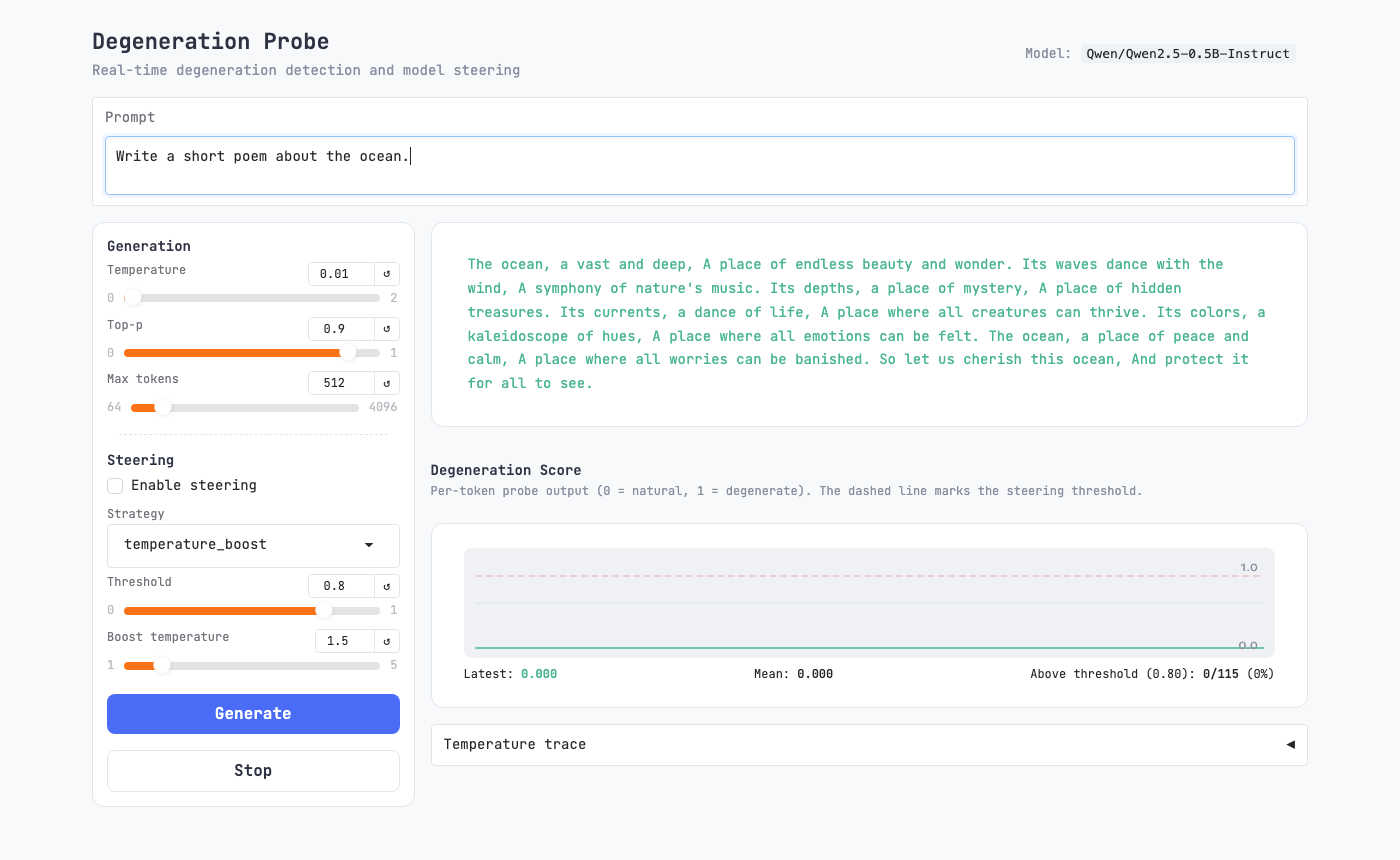
\includegraphics[width=0.95\textwidth]{ui_layout_cropped.png}}
\end{figure}

\q{Are the use cases realistic?}
Yes. All four are executable today against a local Qwen-0.5B or the
Clariden Apertus-8B worker:
(1)~\emph{see} degeneration at low temperature with steering off;
(2)~\emph{fix} it by turning steering on;
(3)~tune sensitivity via the threshold slider;
(4)~swap between local and remote workers without UI changes.

\q{Are the use cases clear and understandable?}
Each maps to a visible state change: tokens redden (1), underlines
appear and the curve bends down (2), next-token colour shifts (3),
the worker badge shows the active model (4). No hidden modes.

\q{Do the interactions serve the intended task?}
The task is observing and steering mid-generation. Every control has
an immediate on-screen response --- token colour, score line, underline,
worker badge --- so the UI is a closed observation loop, not a form
submission. Slider changes ride the open WebSocket and show up on the
next token rather than requiring a regenerate.

\section*{Aesthetics}

\q{Use of color: helpful, harmonious, readable?}
Palette \;
\textcolor{uiSafe}{$\blacksquare$}\,safe\;
\textcolor{uiMid}{$\blacksquare$}\,mid\;
\textcolor{uiDanger}{$\blacksquare$}\,danger\;
\textcolor{uiSteered}{$\blacksquare$}\,steered\;
\textcolor{uiAccent}{$\blacksquare$}\,primary action.
Hue is reserved for data (probe score and steering); chrome
(bg \texttt{\#F8F9FB}, card \texttt{\#FFFFFF}, border \texttt{\#E2E6EA})
follows the lecture's rule \emph{lighter, less saturated colours for
larger areas} so the small data marks pop. Dark text (\texttt{\#2D3142})
on light background holds ${\approx}13{:}1$ luminance contrast, well
above the lecture's 3:1 text rule; no dark-on-dark anywhere. Steering
adds a second channel (underline) so red-green colour-blind users
($\approx$10\% of males per lecture) still see intervention points.

\q{Does the design follow the perception principles from the lecture?}
\begin{itemize}
  \setlength{\itemsep}{0pt}
  \item \emph{Pre-Attentive Processing / Popout}: hue encodes probe
  score only --- a red token is detected in ${<}250$\,ms without
  scanning. Never used as decoration.
  \item \emph{Visual channel rankings} (Munzner): the quantitative
  trend uses \emph{spatial position}, the top-ranked magnitude
  channel (``ranks high for both expressiveness and effectiveness'');
  earlier bar sparklines were replaced for exactly this reason.
  Position is also reserved for the most important information
  (score over time), per the lecture's rules-of-thumb slide.
  \item \emph{Gestalt laws}: \emph{Proximity} + \emph{Common Region}
  group controls into Generation / Steering cards; \emph{Similarity}
  of slider shape signals they are the same kind of control;
  \emph{Connectedness} of the score line overrules proximity, so the
  curve reads as one trend.
  \item \emph{Redundant visual encoding}: steering = hue + underline;
  threshold = colour + dashed style --- survives colour-blindness and
  greyscale printing, per the lecture's colour-vision guidelines.
  \item \emph{Expressiveness \& effectiveness}: we show all and only
  the task-relevant variables (score, threshold, steered-ness, active
  model); no chart junk, no 3D, no inflated \emph{Lie Factor}.
  \item \emph{Tight feedback}: slider changes reach the worker over
  the open WebSocket and show up on the next token, keeping the
  perception loop under the attentive-processing threshold.
\end{itemize}

\end{document}
